\begin{figure*}[t]
\centering
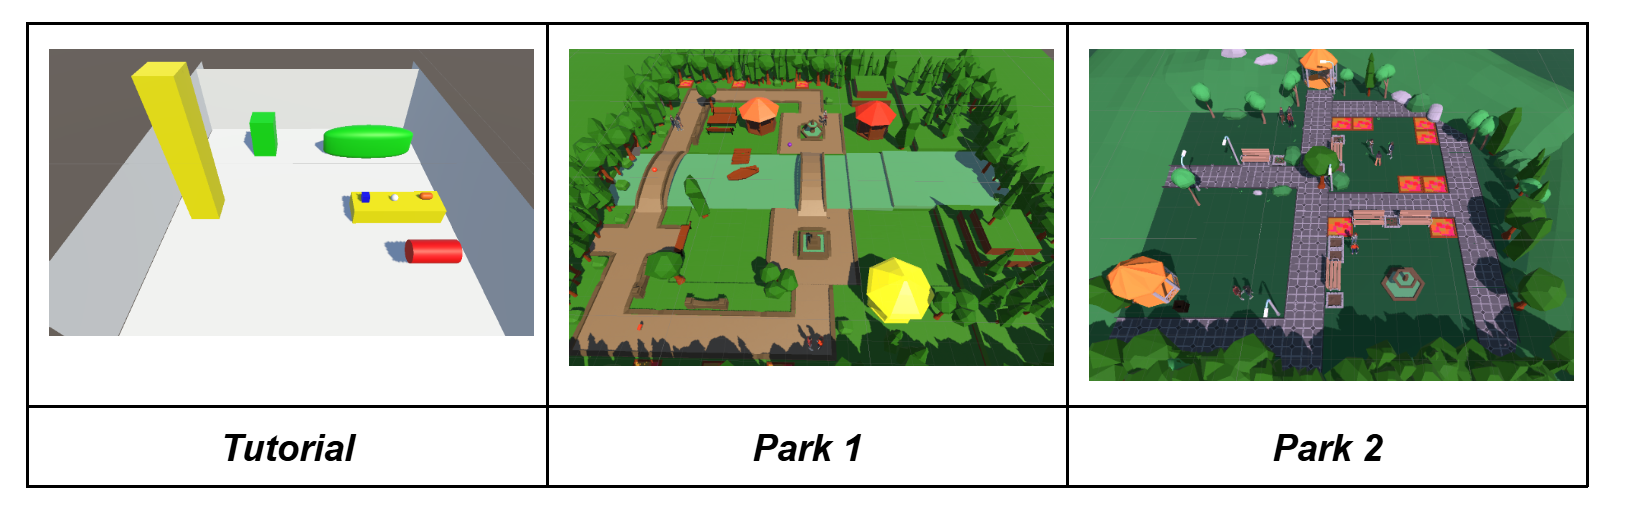
\includegraphics[width=350pt]{virtual_environments.png}
\caption{\label{fig: Virtual Environments} The three virtual environments used in the study. From left to right, the Tutorial contains various simplistic 3D objects such as yellow and green cubes, Park 1 contains a large river and several colorful gazebos, and Park 2 contains colorful flower beds and a series of benches for resting throughout the park.}
    \Description{A table with three images of the virtual environments used in the study. On the far left is an image of the tutorial room, a simple white room with various geometrical shapes, including a yellow, horizontal cube acting as a table with three interactable shapes resting on it. In the middle is a screenshot of the first park with trees scattered about and a river cutting through, populated by stone walkways and bridges, two water fountains, three gazebos, and three groups of avatars. On the right is a screenshot of the second park, a brightly-lit park with stone tile walkways around a few square patches of grass, two gazebos, and a group of avatars gathered for a dance party.
}
\end{figure*}